
\section{Search for pre-coincidence}
\label{sec:precoince}

Because the line count would in this case be smaller than in the unfiltered case it is of interest to investigate whether some of the \Kr\ decay caused events might be possible to recover.
The absolute number of events filtered out by the LAr veto in the energy range of 509 to 519 keV is 1728.
This number is too big to look at every individual case manually.
\\

Luckily, the excited \nuc{Rb}{85m} state has a half life of 1.015 \(\unit{\mu s}\).
This means that one should be able to measure pre-coincedence events of the beta creating scintillation light before the germanium detector event.
This way one can hopefully identify the majority of events created by \Kr\ decays over the rest of the filtered signals.
For this purpose, the events used for the investigation must be limited to those that have a negative time difference between the germanium events and the photomultiplier signal.
The time difference for each individual liquid argon events is already analyzed and stored in the vector $"$triggerLAr$"$ of the Tier3 data set.
This vector has the same number of dimensions as photomultipliers and each entry is indexed with the corresponding input channel of one.
The entries of this vector are again vectors that store the time difference for each signal that triggered the LAr veto in the corresponding channel.
Since only the earliest trigger event of the photomultiplier is of interest for the analysis,  for reasons of simplicity only the first entry of this internal vector will be used as they are ordered in ascending order.
From this point, only events where at least one photomultiplier has measured a negative time difference are used for the recovery analysis.
\\

In addition, as already mentioned earlier, the energy of the released beta electron is very low.
This means that one can expect from a \Kr\ decay into an excited state of \nuc{Rb}{85m} that only a small number of photomultipliers should measure a signal.
This is because the effective scintillation yield of the \gerda\ setup is about 60 phe/MeV.
With a mean energy of 47.65keV one can expect that to measure 1 to 4 photons per decay.
thereforee, only events with a maximum of four different triggered photomultipliers are used in the further analysis.
This amount of coincedently triggered photomultiplier leaves still a lot of events.
But due to the fact that later in the analysis a manually investigation into the individually measured events will be performed the filter can be a little coarser here.
\\

\begin{figure}[t!]
	\centering
	\ifmakefigures%
	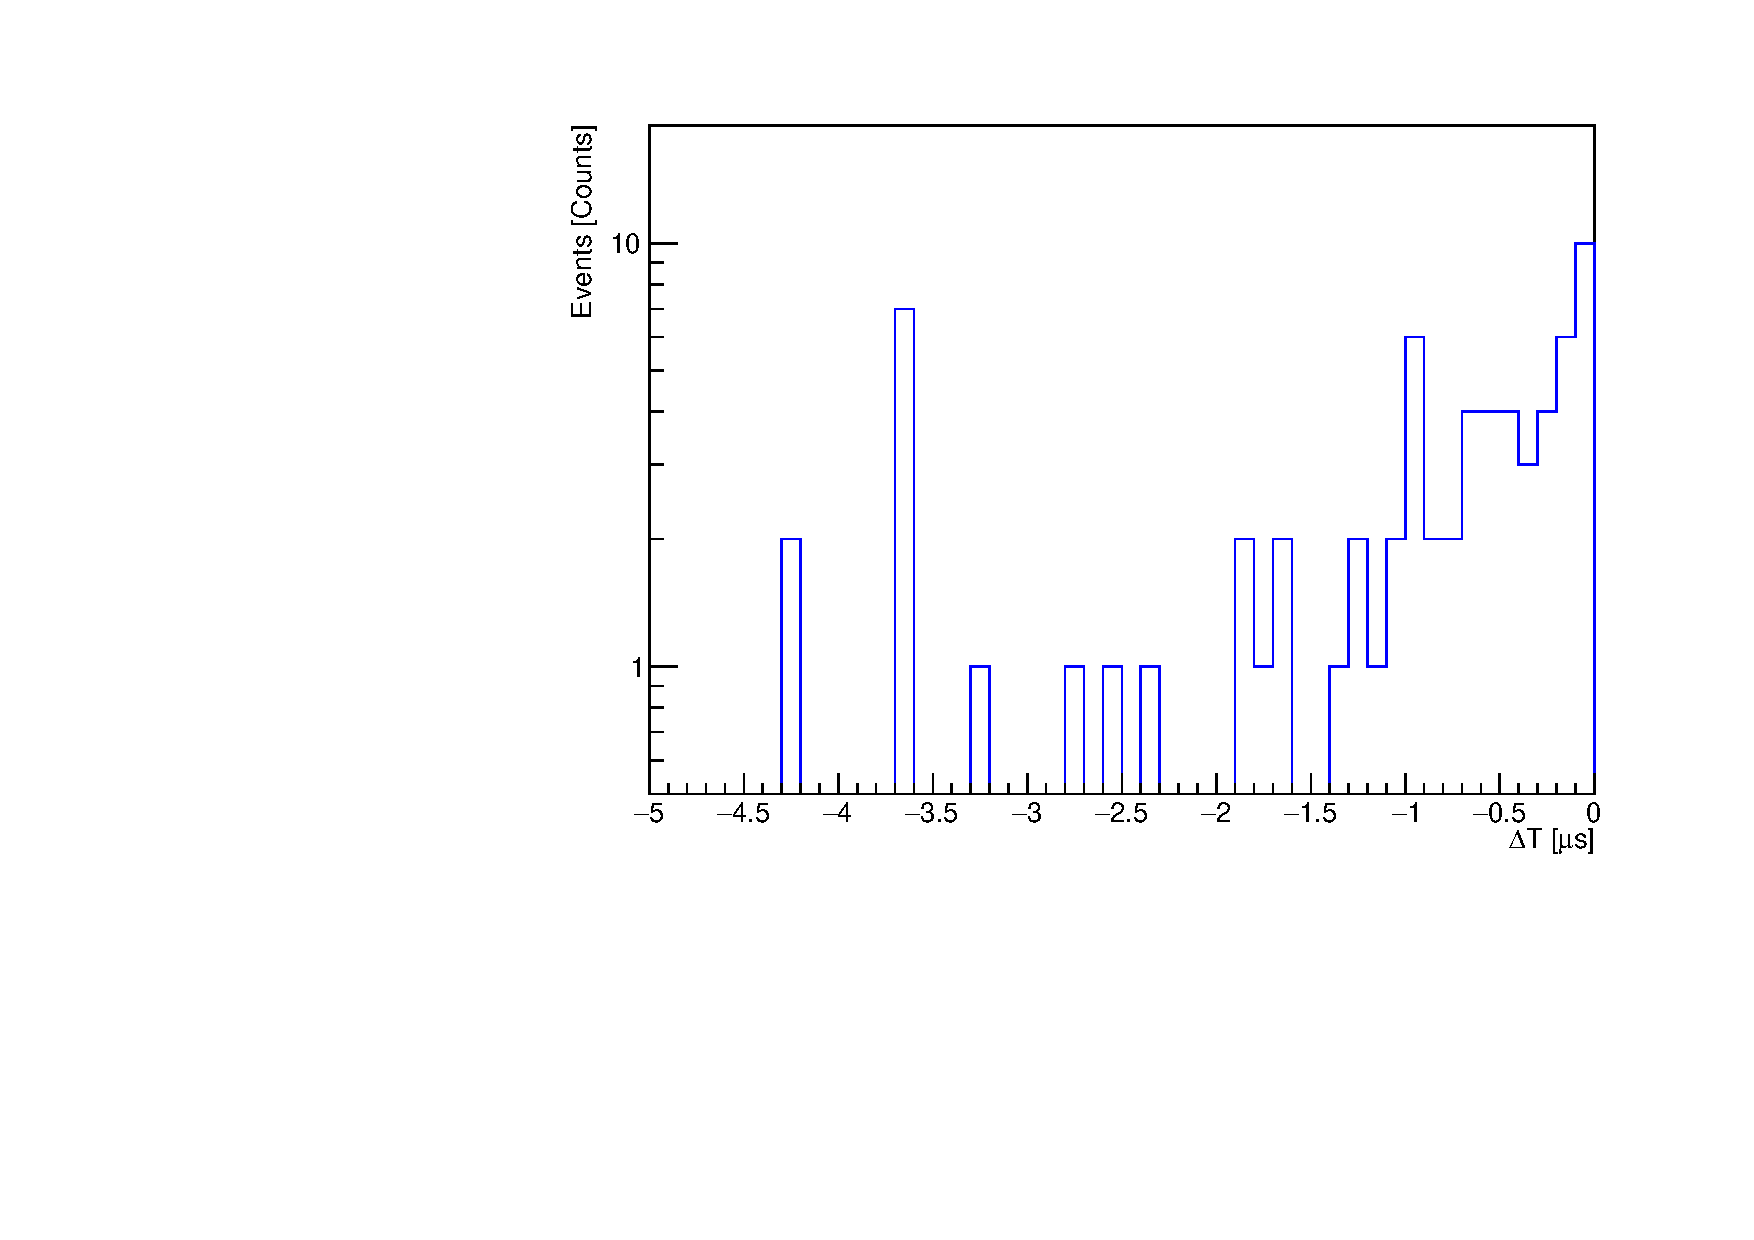
\includegraphics[width=100mm]{./Bilder/TriggerTimeOnly4.pdf}
	\fi%
	\caption{
	    Counts plotted over the time difference between the germanium detector event and the signal in the photomultipliers.
	    The range of the plot only shows the negative time difference from -5 to 0 $\mu$s.
	    This means that all events creating this plot measured a photomultiplier signal before an germanium detector signal.
	    Due to \nuc{Rb}{85m}'s half life of 1.015$\mu$s an exponential increase should be identifiable but with the low amount of counts no statement can be made. 
	}
    	\label{fig:Trigger4}
\end{figure}

Applying these two restrictions to the LAr veto filtered events and using from those only those photomultiplier events with a signal strength of at least 0.5 phe results in a distribution as shown in figure \ref{fig:Trigger4}.
Only the signals that have measured at least 0.5 phe are of interest because they had the necessary intensity to trigger the LAr veto. 
The x axis is the time difference of the events in the photomultipliers from the signal measured in one of the Germanium detectors.
Theoretically it should be possible to see a exponential increase from the negative scale towards a vanishing time difference.
But due to the small number of events, it is basically impossible to make any statements about the course of these events.
\\

Nevertheless, the number of events of interest was reduced from 1728 to only 55.  
These remaining events can now be manually examined with a software called GerLa.
This tool allows one to search for a specific events and see all recorded signals of the Germanium detectors and the photomultipliers around the time frame of this event.
\\

With this program one can now perform a manual filter.
This can be done by looking at the remaining 55 events individually and decide whether to reject an event or not using a specific protocol.
This protocol consists of rejecting every event that has a combined light intensity of over 5 phe and every event that only has a negative time difference in a signal weaker than 0.5 phe.
The upper limit of the light intensity originates again from the expected number of photons as described earlier.
\\

\begin{figure}[t!]
	\centering
	\ifmakefigures%
	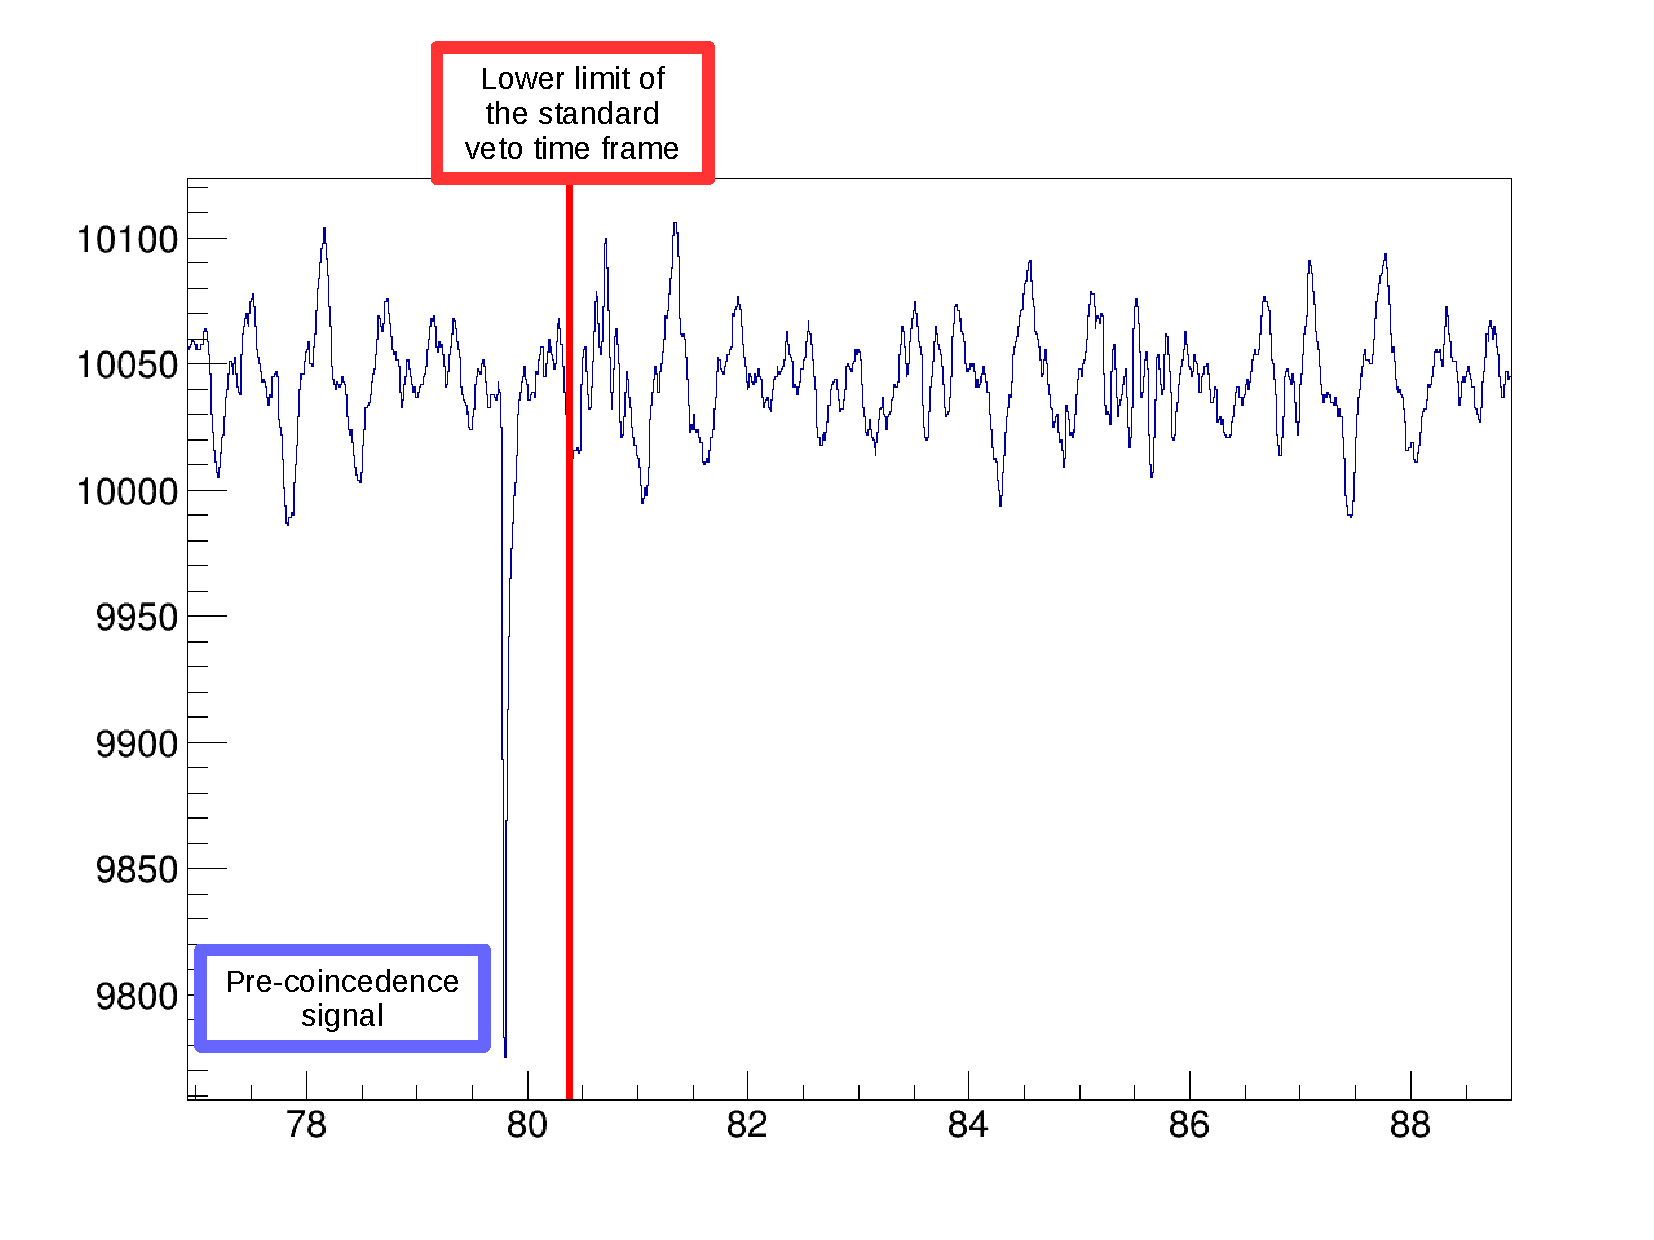
\includegraphics[width=100mm]{./Bilder/BeispielSignal.pdf}
	\fi%

	\caption{
    The recorded signal of photomultiplier tube P4 in event 1614036. 
    In it is the raw energy signal plotted over the recorded time frame. 
    The blue line indicates the moment in time in which an event in one of the germanium detectors was measured. 
    From it one can see that the photomultiplier signal occurred before the germanium detector signal.   
    }
    	\label{fig:BeispielSignal}
\end{figure}

While going through each of the 55 events, it quickly was realized that this procedure does not work as well as we hoped it would.
From the remaining 55 only a handful of events were unambiguous enough that one can claim that the photons must originate from expected beta electron.
After this much filtering it can assume the few that were found are probably all in fact caused by a \Kr\ decays.
Signals like the one shown in figure \ref{fig:BeispielSignal} are a rare example of an almost model signal that were expected to be measured.
The great majority of other events were either background events in the SiPM that seem to randomly triggered the LAr veto or the combined signal strength was much higher than 5 phe.\\

This leads to the conclusion that the majority of signals in the photomultiplier with a negative time difference were in fact not caused by the beta electrons scintillation light but rather coincidences with other signals.
This means it is practically impossible to recover any of them with the process presented here.

The recovery attempt has failed.
\\

Nevertheless we are still able to make some qualitative estimations about why approach might not have worked. 
The problem of this recovery attempt seems to be that the majority of events detected with a negative time difference are in fact background events.
This conclusion came from the fact that almost none of the events investigated have shown the features we expected from them.

An indicator for this can be seen in the fact that the majority of light signals have been measured in the PMTs.
As it will be shown in section \ref{sec:MonteCarlo514}, basically all of the decays that created a measurable 514keV event have happened in the vicinity of the detectors.
The detectors themselves should already block some of the light but when a photon is detected in a photomultiplier it would most likely be a SiPM.
This is because the nylon fibers surrounding the germanium detectors are more likely to absorb and guide the scintillation light to the SiPM than a photon to reach a PMT above or below the detector arrays.
Now that the majority of the detected light events are measured in the PMTs it is very unlikely that these are caused by a \Kr\ decay.

%That the majority of the 
%This might also be able to be seen from figure \ref{fig:AntiLArBEGes} and \ref{fig:AntiLArCOAX}.
%From them one was able to see that the LAr veto also filtered out some of the 514keV line events.
%But from it can also be seen, that the ratio of events filtered out at the 514keV mark over the non filtered value [$N_{\unit{vetoed}}(514\unit{keV})/N_{\unit{unfilered}}(514\unit{keV})]$ is of about the same size as in the background area whereas the positron electron peak shows much higher ratio.
%Considering this the peaks in \ref{fig:AntiLArBEGes} and \ref{fig:AntiLArCOAX} probably came to be  due to the same relative amount of events have their liquid argon veto triggered because of background events.
Because of this it is rather questionable whether the LAr veto is even a good identifier to use when it also filters out events in which background can trigger the veto.
A satisfactory answer however will only be able to obtain through a quantitative analysis which will be performed in the following chapter.
\\
